% decide: stoichiometry model/ terminology for the two models and correct in chapter 4
\label{chap:results}
In this chapter, the results of the implementation of \aclp{spdm} will be analysed and discussed. Results will be compared on two different levels: both the recalculated inventories and the \aclp{GWI} of processes and products will be taken into account.


\section{Comparison of Inventories of Production Processes}
\label{sec:inventories}
First, the inventories of the recalculated production processes will be compared. More specifically, the total heat use and the reactant mass flows will be analysed.

\subsection{Total Heat Use}
Heat in chemical processes is assumed to equal the sum of the energetic values of steam and natural gas passing the system boundary of the single chemical process as both represent the most important energy sources for heat generation in chemical processes \cite{Boustead.1999}. Steam is assumed to have a specific energy content of 2.75 MJ/kg \cite{Althaus.2007}. The criterion of heat is used, for it is a major driver of the \acl{GWI} of chemical products. 42 \% of the carbon feedstock used by the chemical industry is used to generate process energy by incineration \cite{InternationalEnergyAgency.2017}, thereby causing the emission of \aclp{GHG}. Simplified process design methods can only be used to calculate the required heat for a process, but not its form, neither its temperature level \cite{Parvatker.2019}. Therefore, this unspecified heat was assumed to be comparable to the combined natural gas and steam use of the industry datasets. Figure \ref{fig:inventories} shows the results of this analysis. Positive values indicate an output of energy, while negative values refer to an energy input. 

\begin{figure}[htp!]
        \centering
        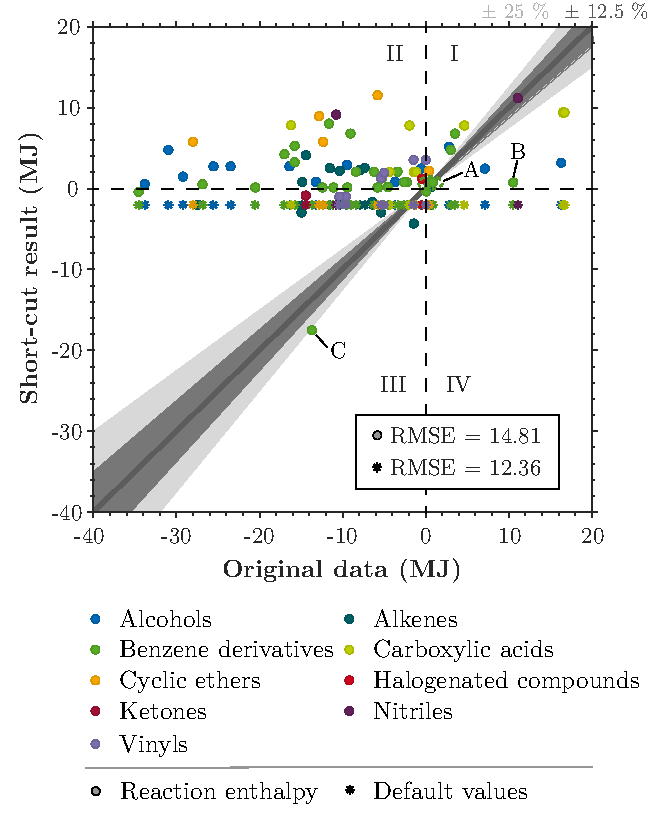
\includegraphics{images/figure_1_clean.pdf}
        \caption{Comparison of the original and recalculated energy output values assumed as steam and natural gas required per one kg of main product. (A) and  (B) mark ethylene- and benzene-based production processes for ethylbenzene with low and high errors, respectively. (C) marks another production process for ethylbenzene that is ethane-based. RMSE refers to the root-mean-square error.}
        \label{fig:inventories}
\end{figure}

\paragraph{Method 1: Stoichiometric Mass Flows and Reaction Enthalpy}
There does not seem to be an overall correlation between the chemical groups and their respective errors. 
\subparagraph{Quadrant I} 
Both the short-cut and original values for the energy outputs are positive. Few points lie in this area in total. Single results are near the 50 \% variance range. One result matches almost perfectly the original value with an error of 0.5 \%: a propane-based acrylonitrile production process. The accumulation of three benzene derivative points near the coordinate origin marked with a dashed green line and the letter A in Figure \ref{fig:inventories} represents three ethylbenzene production processes. All of them have the same underlying stoichiometric formula and therefore form a horizontal line at the value of 0.76 MJ/kg, which means that the underlying reaction is exothermic as the values of method one equal the reaction enthalpy\footnote{it is explicitly remarked that the sign definition of the reaction enthalpy is contrary of the one used in inventories and in Figure \ref{fig:inventories}.}. The original datasets, however, are widely spread: tree of them match this value with relatively low errors (-51.5 \%,	-62.4 \%	 and 13.4 \%, respectively) while another process (B) has an original energy value of 10.54 MJ/kg. While the processes (A) require natural gas and have an output of steam in similar value ranges due to the internal incineration of residuals as fuel, the process (B) both delivers high amounts of natural gas and steam with a value that is more than one order of magnitude higher than the reaction enthalpy of the underlying process. While this process operates at much lower temperature and pressure levels than the processes (A) and therefore, less energy is used internally for heating and pressurizing, it is still a surprisingly high value that, when considering the energy balance of the process, can only be achieved if the inputs have a much higher temperature than the products in the effluent stream. This might be the case in a specific chemical production facility that is interlinked with upstream processes that deliver the input materials at high temperatures as a result of the previous reactions.

\subparagraph{Quadrant II}
In this quadrant, the new inventories have an energy output, meaning that the processes are exothermic, while the original processes require an energy input. Most of the points representing the compared inventories are located in this area with overall large discrepancies between the original and the recalculated values. The reason for this likely is the fact that the reactor -- and therefore the reaction enthalpy -- only represents one element of the whole process. Often, heat is needed for distillation and for preheating the reactants to reaction conditions, even if the reaction is exothermic. In this latter case, surplus energy might be integrated to reduce the heat demand. 

An example of this effect is the production of \acl{BPA}. While the underlying stoichiometry results in a reaction enthalpy of 0.14 MJ/kg (and therefore forming a horizontal line), the original values range from -20.5 MJ/kg to -5.72 MJ/kg, depending on the reaction details such as temperatures, pressures, the number of reaction steps and distillation or purifying process steps; although only one synthesis route for the production of \acl{BPA} is industrially used \cite{Fiege.2000}. This underlines the importance of the reaction conditions that should be taken into account when the required energy for a process is estimated, as previously stated by Jiménez-González et. al.  \cite{JimenezGonzalez.2000}.  

\subparagraph{Quadrant III} 
In this area, both the short-cut and original values reflect an overall energy input. This means that these are endothermic reactions. The overall errors in this area are very high. 
One case (marked with the letter C in Figure \ref{fig:inventories}) matches with a relatively low error of 27.9 \%: another production process for ethylbenzene that is ethane-based. The required energy for this highly endothermic reaction with a reaction enthalpy of $\Delta h_R = -17.51$ MJ/kg to take place is supplied to the process in the forms of (\textit{i}) 15.7 MJ/kg steam, natural gas and electric energy and (\textit{ii}) by an excess of the reactants ethane and benzene that are burned internally as reaction residues, thereby providing around 4.5 MJ/kg (lower heating values according to NIST Chemistry WebBook \cite{NationalInstituteofStandardsandTechnology.2018}).

\subparagraph{Quadrant IV} 
Here, the reactions are endothermic, but the industry datasets report an energy output. There is one single case in this area: a dimethyl terephtalate production process using p-xylene. The difference in energy is supplied to the system in the form of electric energy.


\paragraph{Method 2: Stoichiometric Mass Flows and Ecoinvent's Default Energy Values}

As the default value of $-2$ MJ steam per kg output is assumed, the points form a horizontal line. Two results are within the 25 \% range and no additional results are in the 50 \% range, representing 3.6 \% of the overall results. Figure  \ref{fig:histogram} shows the distribution of the combined heat output values assumed as natural gas and steam of the reference datasets. This distribution equals the density of the points of Method 2 in Figure \ref{fig:inventories}. It clearly depicts that the individual values are widely spread, with a standard deviation of 11.34 MJ and a mean value of $-5.98$ MJ. Consequently, using one default value must lead to high errors.

\begin{figure}[htp!]
        \centering
        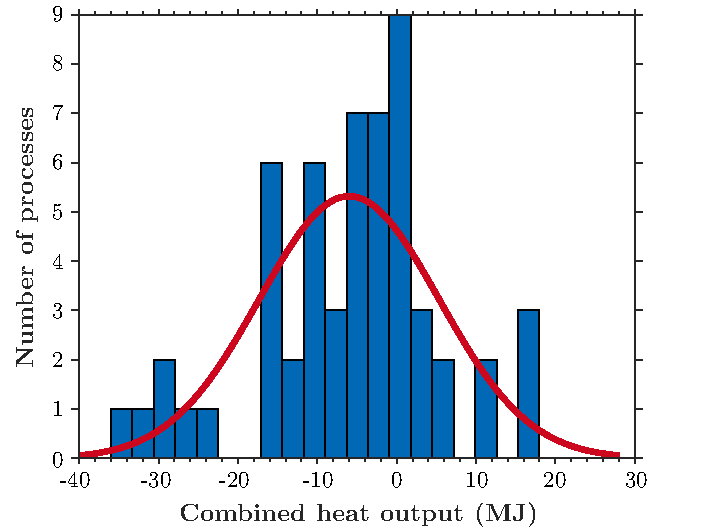
\includegraphics{images/histdist.pdf}
        \caption{Distribution of the combined heat output values assumed as natural gas and steam of the reference datasets}
        \label{fig:histogram}
\end{figure}


\subsection{Reactant Mass Flows}
The following comparison is carried out to assess the accuracy of the estimation of reactant mass flows using stoichiometric equations and the assumption that 5 mass-\% of the inputs are burned. Figure \ref{fig:masses} shows the result of this comparison. Each point refers to an individual mass flow in one process. As both new models use the same method to calculate reactant flows, their results equal.


\begin{figure}[htp!]
        \centering
        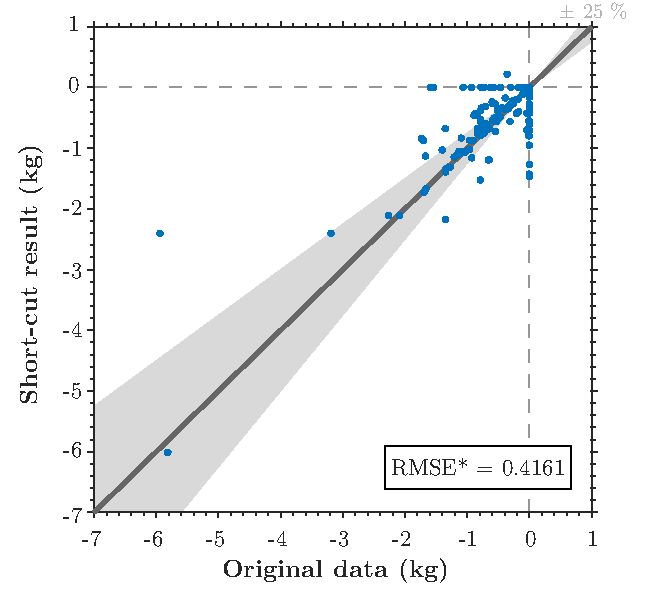
\includegraphics{images/masses.pdf}
        \caption{Comparison of the original and recalculated reactant masses per one kg of main product. The asterisk refers to the set of points not lying on the $x=0$ or $y=0$ lines. RMSE refers to the root-mean-square error.}
        \label{fig:masses}
\end{figure}

40.61 \% of points lie on the $x=0$ or $y=0$ lines. These are cases in which the original model has a mass input, but there is no input of the same chemical in the same process in the new models ($y=0$) and vice-versa. This high percentage of values that only exist in one of the two compared models may indicate several aspects. Firstly and most importantly, the system boundaries of the original and the recalculated processes may not match. This means that the  reactants may differ because of the in- or exclusion of upstream reactions. In the case of very limited data about the reference process, these points may therefore indicate a false synthesis route. Secondly, by-products may be excluded in the reference dataset due to different treatment of these products in industrial processes. 

In one case, the new models have an output of a chemical, while the original dataset uses the same chemical as an input. When only considering non-zero points, the overall derivatives between the estimated mass flows and the original ones are low. 18.38 \% of the points lie within a 5 \% error range, 33.09 \% and 50.74 \% in 10 \% and 25 \% ranges, respectively. For the same set of points, the root-mean-square deviation is 0.4161 kg. 


\section{Comparison of the Impacts of Production Processes}
\label{sec:impacts}

As this thesis is mainly motivated by the need of the chemical industry to reduce its \acl{GHG} emissions, the impact ``ILCD\footnote{The International Reference Life Cycle Data System (ILCD) established by the European Commission, Joint Research Centre, Institute for Environment and Sustainability (JRC - IES) \cite{EuropeanCommissionJointResearchCentreInstituteforEnvironmentandSustainability.2012b}} 1.0.8, 2016, midpoint, climate change, GWP 100a'' \cite{EuropeanCommissionJointResearchCentreInstituteforEnvironmentandSustainability.2012d} was used for the following comparison. The values indicate the \acl{GWI} of an activity\footnote{an activity can be any kind of transformation, production or service defined within the functional unit of the LCA.} in kg CO$_2$-eq based on the characterization factors for elementary flows to the environment published in the Fourth Assessment Report of the Intergovernmental Panel on Climate Change \cite{IPCC.2007}. Inititally, the \aclp{GWI} of all processes included in the database are compared. This comparison is depicted in Figure \ref{fig:impacts all}. Blue dots refer to the model using the reaction enthalpy based model, while red ones refer to the model using Ecoinvent's default energy values.


\begin{figure}[htp!]
        \centering
        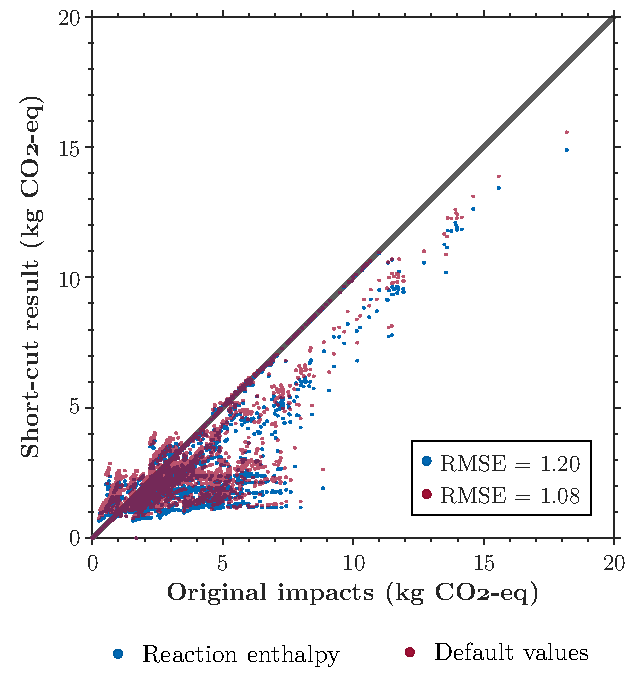
\includegraphics{images/complete_all.pdf}
        \caption{Comparison of all original and recalculated impacts per one kg of main product output included in the ``cm.chemicals'' database \cite{CarbonMindsGmbH.2020}}. RMSE refers to the root-mean-square error.
        \label{fig:impacts all}
\end{figure}

The figure shows that there is a multitude of effects that can be observed with impacts being under- and overestimated in different cases. Some impacts stay equal and seem to be uninfluenced by the changes. The root-mean-square errors of both models are greater than 1 kg CO$_2$-eq with the the second model (RMSE$_2 = 1.08$ kg CO$_2$-eq) performing slightly better than the reaction enthalpy-based model (RMSE$_1 = 1.20$ kg CO$_2$-eq). This means that both models distort the results of the database substantially. To understand some effects in detail, two processes for the production of 1,4-butanediol and vinyl chloride, respectively, will be analysed in detail. For butanediol, a single process based on the reactants acetylene and formaldehyde is studied in detail. It is one of five existing production processes for butanediol.
Figure \ref{fig:butanediol} shows the comparison of the impacts of these five processes. 


\begin{figure}[htp!]
        \centering
        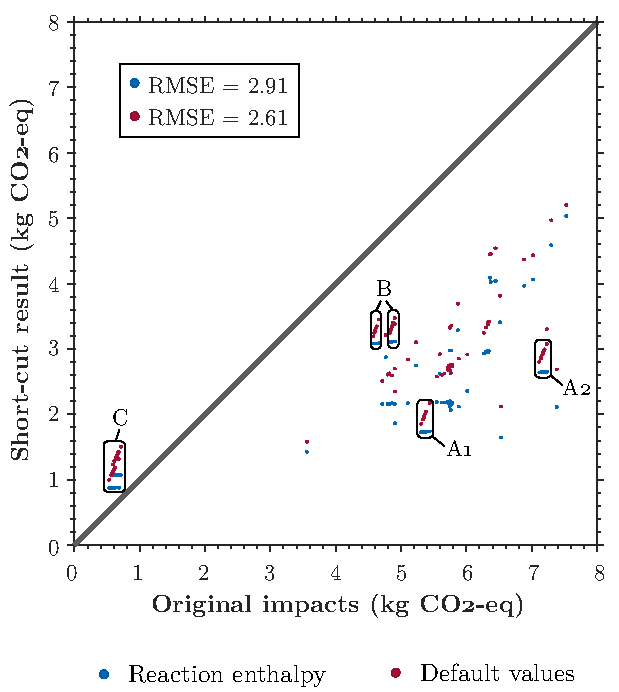
\includegraphics{images/butanediol.pdf}
        \caption{Comparison of the original and recalculated impacts per one kg of 1,4-butanediol for all existing production processes. The letters refer to the following processes: (A) 1,4-butanediol from aetylene and formaldehyde, (B) 1,4-butanediol from maleic anhydride, (C) 1,4-butanediol from butane via maleic acid hydrogenation. RMSE refers to the root-mean-square error.}
        \label{fig:butanediol}
\end{figure}

It can be observed that most impacts are underestimated. There are only a few cases in which the impact is overestimated, all representing the same process. There are patterns or constellations of points representing the different production processes. To understand what the original and recalculated impacts include and why this result is obtained, a contribution analysis in performed. Figure \ref{fig:contribution butanediol} depicts the results of this analysis for two producing regions, Argentina and Belgium, and for the original and two new LCA databases.


\begin{figure}[htp!]
        \centering
        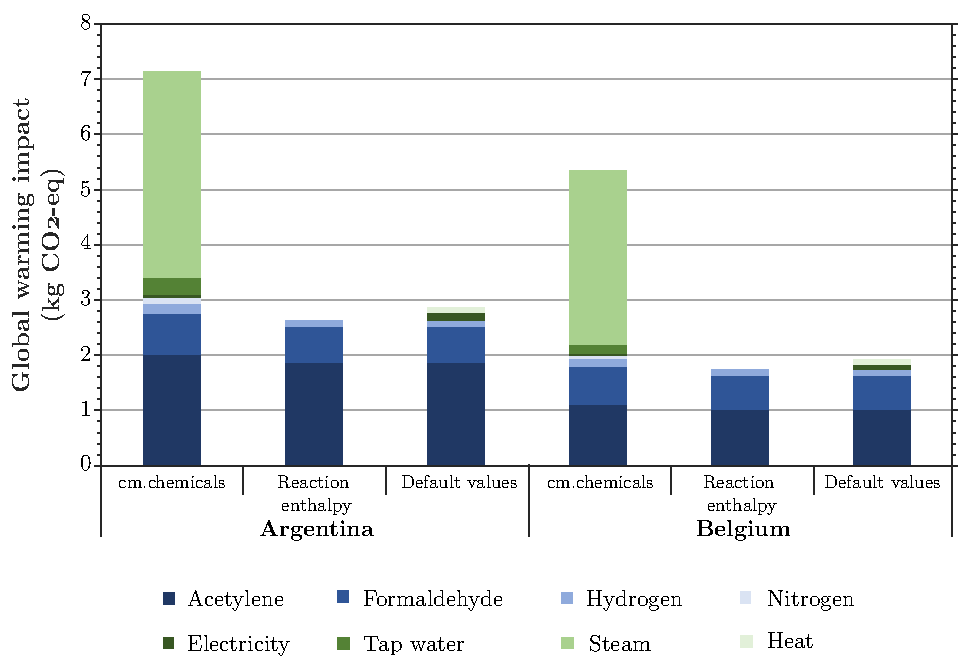
\includegraphics[width=\textwidth]{images/contribution_butanediol.pdf}
        \caption{Contribution analysis of the original and recalculated impacts per one kg of 1,4-butanediol produced by a process based on acetylene and formaldehyde}
        \label{fig:contribution butanediol}
\end{figure}

These results show how the different impacts are composed. Firstly, there is a difference of 1.8 kg CO$_2$-eq between the impacts of the original process when it is used in Argentina compared to its usage in Belgium. This means that in Belgium, the carbon footprint of this production is 25 \% lower. This difference is due to higher impacts of the raw materials acetylene, formaldehyde, hydrogen and nitrogen and the process utilities electricity, tap water, steam and heat. Most importantly, the impact of acetylene is almost twice as high in Argentina than in Belgium. 

In the same country, the impacts calculated using the two new models are by far underestimated when compared to the original impact. The figure also shows that this is mainly due to the drastic underestimation of the steam demand, while reactant-related emissions are very accurate and only almost 10 \% underestimated. 

In the reaction enthalpy based model, the process was calculated to be exothermic. Therefore, the process has undergone allocation, because the surplus energy occurred in the inventory as second output. Additionally, the electricity demand is underestimated. The default heat and electricity values used in the second model are by far too low compared to the real process. Therefore, the impacts are underestimated in both cases.

In all models, all inputs for this process are directly supplied by aggregated  processes from the Ecoinvent database. But these processes only exist for the two regions ``RER'' (Europe) and ``RoW'' (Rest-of-World), except for the electricity supply which exists for most countries individually \cite{Ecoinvent.2020}. This is the reason for similar patterns to occur in Figure \ref{fig:butanediol}. These patterns all represent the same process; but their impact is vastly dependent of their classification regarding the two geographical categories existing in Ecoinvent for the named inputs as has shown the example of Argentina and Belgium. As electricity is the only input that is supplied with processes of high geographical resolution, the points for one model form a line rather than a more complex distribution. It is then its recalculated value that changes the gradient of that line. The closer this value is to the original value, the closer the gradient is to one. This is because, when considering two neighboring points of the same model (A and B) in the same constellation (representing two ``RER'' or ``RoW'' countries, such as two points in the area A$_1$ in Figure \ref{fig:butanediol}), it equals the ratio of the difference in GWI of the new model (on the $y$-axis) divided by the difference in GWI of the original model (on the $x$-axis),
$$
c = \frac{\Delta \mathrm{GWI}_\mathrm{new, \ y}}{\Delta \mathrm{GWI}_\mathrm{original, \ x}}.
$$
These differences equal the difference in GWI of the electricity used because the GWI of all other inputs do equal for both countries in the same region and their deltas are 
$$
\Delta \mathrm{GWI}_i = \sum_j \Delta \mathrm{GWI}_{i, \ j} = \Delta \mathrm{GWI}_{i, \ \mathrm{electricity}},
$$
where $i$ indicates the model used (and can therefore be ``new'' or ``original'') and $j$ refers to the different mass- and energy flows contributing to the total GWI of the process.
The GWI of the electricity used in the same process but in two different countries is the product of the electricity value in the corresponding inventory and the specific GWI of electricity in kg CO$_2$-eq/MJ in the two countries,
$$
\Delta \mathrm{GWI}_{i, \ \mathrm{electricity}} = e_{i} \cdot \left( \mathrm{gwi}_{\mathrm{electricity}, \ \mathrm{A}} - \mathrm{gwi}_{\mathrm{electricity}, \ \mathrm{B}}  \right),
$$
where A and B refer to the neighboring countries. Therefore, the gradient becomes
$$
c = \frac{\Delta \mathrm{GWI}_\mathrm{new, \ y}}{\Delta \mathrm{GWI}_\mathrm{original, \ x}} = \frac{e_{\mathrm{new}} \cdot \left( \mathrm{gwi}_{\mathrm{electricity}, \ \mathrm{A}} - \mathrm{gwi}_{\mathrm{electricity}, \ \mathrm{B}}  \right)}{e_{\mathrm{original}} \cdot \left( \mathrm{gwi}_{\mathrm{electricity}, \ \mathrm{A}} - \mathrm{gwi}_{\mathrm{electricity}, \ \mathrm{B}}  \right)} = \frac{e_{\mathrm{new}}}{e_{\mathrm{original}}}
$$
and therefore can vary in the ranges
$$
c = 
\begin{cases}
c \in [0,1),          & e_\mathrm{original} > e_\mathrm{new} \\
1,                  & e_\mathrm{original} = e_\mathrm{new} \\
c \in (1, \infty),     & e_\mathrm{original} < e_\mathrm{new}.
\end{cases}
$$
This means that if the electricity value is overestimated, the gradient gets larger than one and if it is underestimated, it gets lower than one. 
As the electricity values of the stoichiometry model are near zero, the gradient of the blue lines is also near zero.
The same effect can be found in the data for the production processes of vinyl chloride, as shown in Figure \ref{fig:vinylchloride}.

    
    
\begin{figure}[htp!]
        \centering
        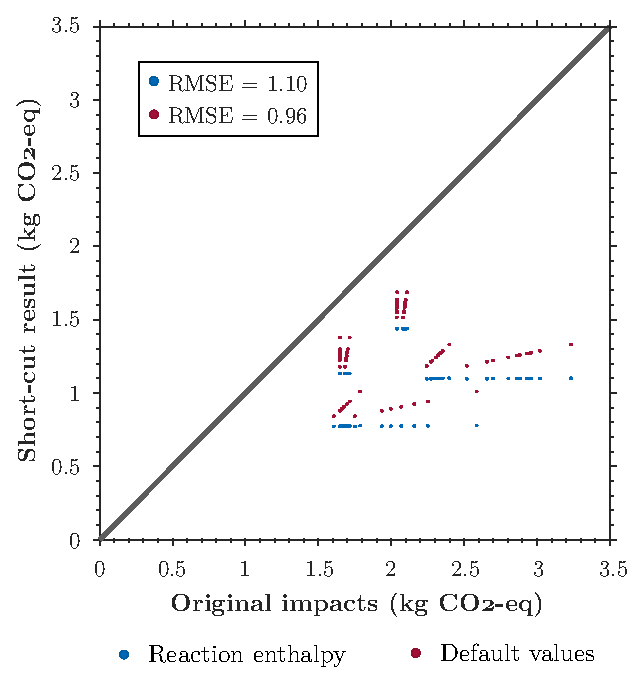
\includegraphics{images/vinylchloride.pdf}
        \caption{Comparison of the original and recalculated impacts per one kg of vinyl chloride for all existing production processes. RMSE refers to the root-mean-square error.}
        \label{fig:vinylchloride}
\end{figure}


As the gradient for one process in one of the two new models can only have one value, the ratio between the recalculated and the original electricity values $c = {e_{\mathrm{new}}}/{e_{\mathrm{original}}}$, it is easily deducible that there must be four production processes for vinyl chloride, as four different gradients appear in Figure \ref{fig:vinylchloride}. Considering the gradients of the red ``lines'', the electric energy value of the underlying simulation model is an underestimate in the case of one process, a good estimate in another process and an overestimate in two processes. 

In the example of vinyl chloride, there is another effect that can be observed. The stoichiometric formulas of the underlying processes all list one or two by-products of the reaction, while the original process has a single output. For example, in a process using ethane, chlorine and hydrogen as reactants, the corresponding stoichiometric formula is \ce{2 C2H6 + 2 Cl2 + O2 -> 2 C2H3Cl + 2 H2O + 2 HCl}, which results in the by-products water and hydrogen chloride. However, in the original dataset, (\textit{i}) none of these by-products are indicated and (\textit{ii}) ethane and oxygen are used in large excess. Both effects result in a non-closed mass balance. Then, in the allocation step, the mass and energy input values are multiplied by the allocation factor ($<1$, because there are by-products) and are therefore much lower for ethane and oxygen than in the original process. This results in fewer emissions related to the production of these two reactants than in the reference dataset, as depicted in Figure \ref{fig:contribution vinylchloride}. The impact of chlorine is almost equal due to the fact that the original dataset's chlorine consumption matches the allocated value of the new datasets. It is likely that ethane is used in excess, because it is burned to provide process heat.

\begin{figure}[htp!]
        \centering
        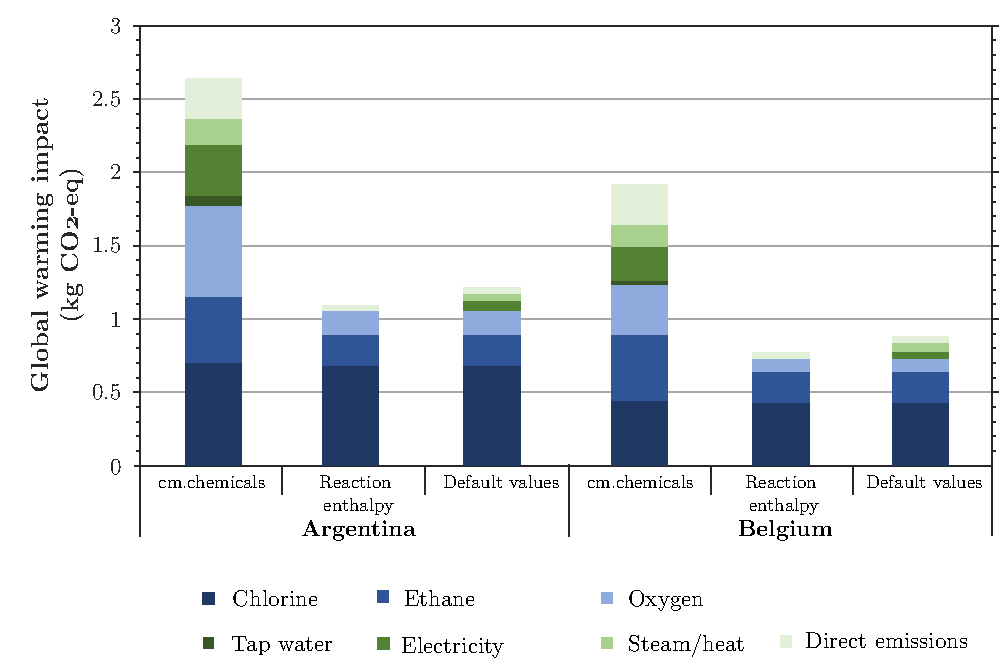
\includegraphics[width=\textwidth]{images/contribution_vinylchloride.pdf}
        \caption{Contribution analysis of the original and recalculated impacts per one kg of vinyl chloride produced by a process based on ethane, oxygen and chlorine}
        \label{fig:contribution vinylchloride}
\end{figure}

